\documentclass[12pt]{article}
\usepackage{float}
\restylefloat{table}
\usepackage{graphicx}
\usepackage{rotating}
\usepackage{color}
\usepackage[dvipsnames]{xcolor}
\usepackage{enumitem}
\usepackage{sidecap}
\usepackage[top=15mm, bottom=15mm, left=15mm, right=15mm]{geometry}
\usepackage{multicol}
\usepackage[dvipsnames]{xcolor}
\usepackage{wrapfig}
\usepackage{hyperref}
\usepackage{courier}

\fboxrule=2pt%border thickness

\pagenumbering{gobble}

\setlength\parindent{0pt}

\begin{document}
\title{DEVILS - Observing and On-site Reduction}
\begin{center}

\begin{figure}
\begin{center}
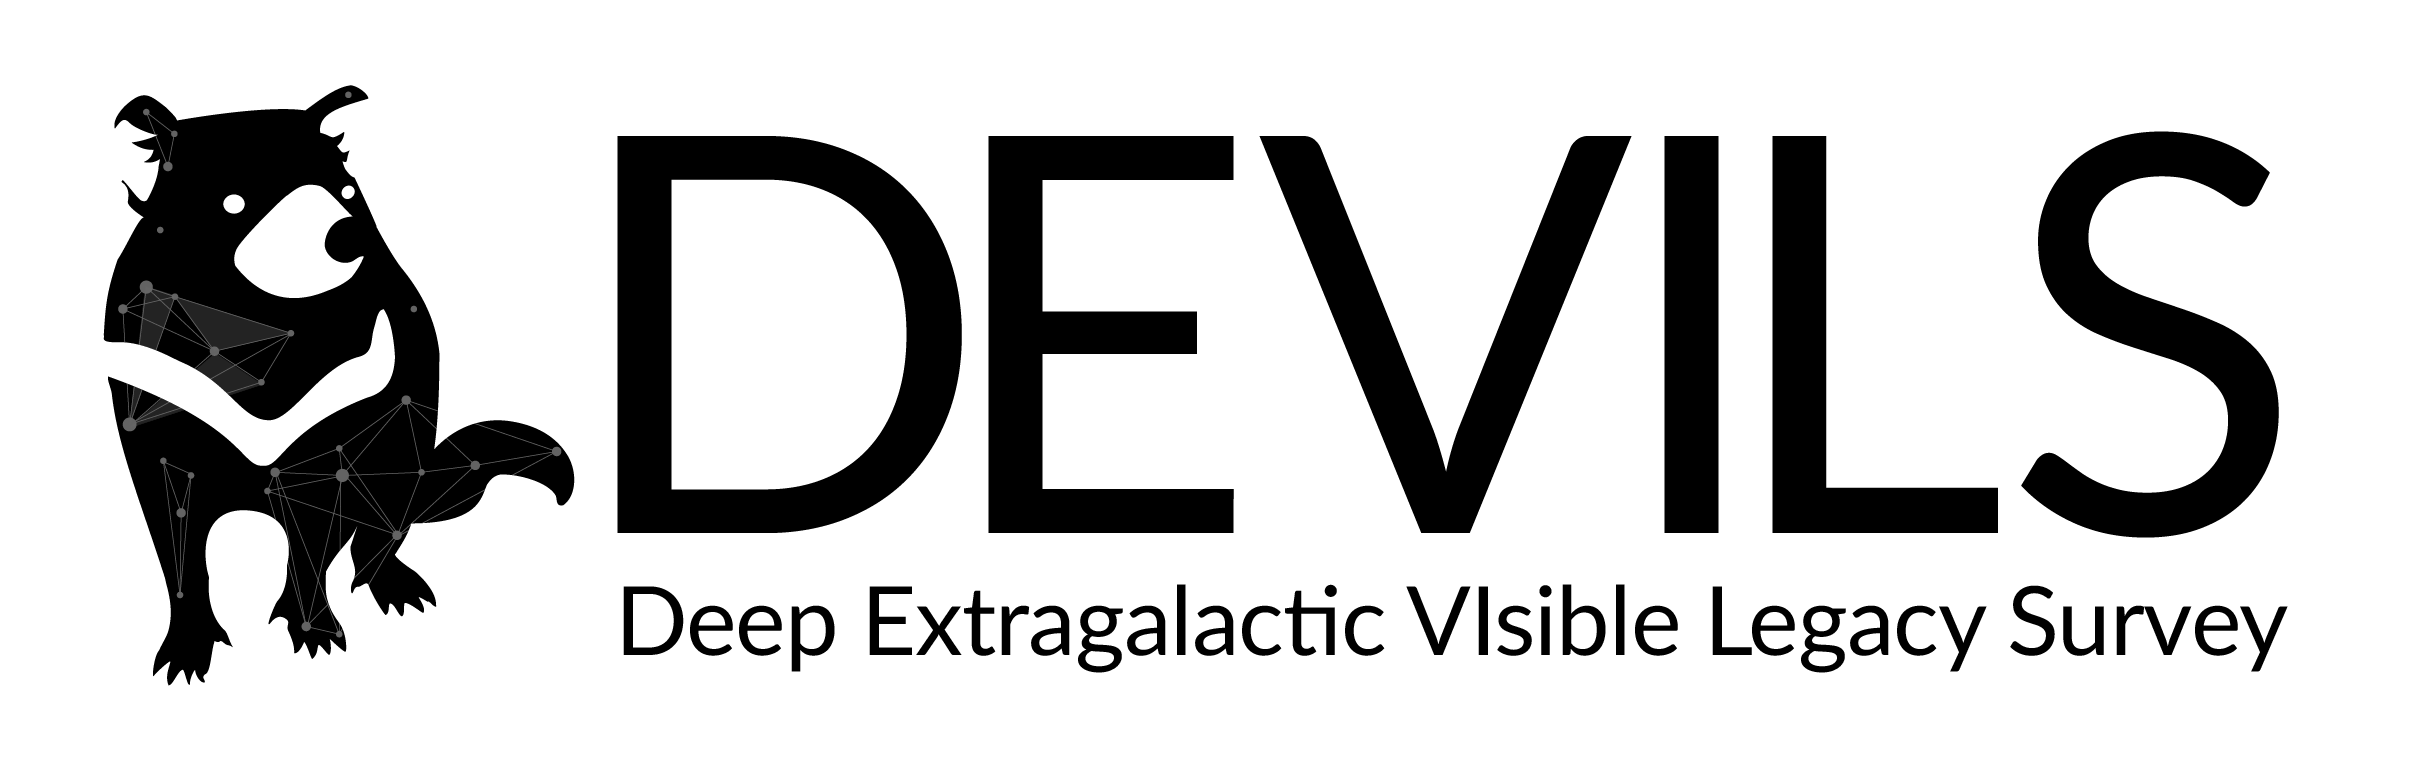
\includegraphics[scale=0.8]{devils-logo_big.png}
\end{center}
\end{figure}

\Huge {\textcolor{PineGreen}{\textbf{Database, Observing and Data Reduction}}}
\Huge {\textcolor{PineGreen}{\textbf{ Version 0.1}}}\\
\Large \textbf{Luke Davies (5/12/2017)}\\
\end{center}
\normalsize


\section{Overview}

The DEVILS observations will be undertaken with the AAT either on-site at Siding Spring or remotely from Perth/Sydney. This document describes the DEVILS database structure and how you interact with it, the observer tasks, and the nightly data reduction and QC processes. In summary, there are two DEVILS databases, each with identical file structure; one at the AAT and one in Perth, with this structure replicated in Sydney by AAO Data Central (ADC) who will be testing new systems and federating the data transfer. The observer will place the raw data in the database at the telescope and the ADC database, this will then get copied to the database in Perth where the data reduction will be performed by the DEVILS Tool for Analysis and Redshifting (TAZ). The reducer in Perth, will produce the new configuration files into the Perth and ADC databases and these will be copied to the AAT database for the next night's observing. At the telescope the observer will perform a manual reduction of the data to check for QC and update logs. A summary of this processes is described in Figure \ref{fig:dataflow} - which will be referred to throughout this document. 

This document provides a detailed description of all aspects of DEVILS observing, for a concise summary of observer tasks see Section \ref{sec:summary}. \textcolor{PineGreen}{\textbf{If you have any queries or questions regarding this document, please contact Luke at luke.j.davies@uwa.edu.au}}\\

     
\section{The DEVILS directory structure}


There is a DEVILS account on the AAT system at the telescope. To access this, first get the password from Luke (luke.j.davies@uwa.edu.au). All of the observer reduction will be done in this workspace in the \textbf{data/reduced\_AAT/} folder. In the following, `$\sim$' will refer to the DEVILS account's home directory. In addition, \% referees to the terminal prompt ($i.e.$ if the document state \texttt{\% configure}, just type \texttt{\% configure}), $>$ will refer to a prompt in R. \\

\textcolor{PineGreen}{\textbf{NOTE: Please be careful not to delete anything from this space! While we have back-ups, it will take some time to reconstruct things.}}\\

The DEVILS data directories has the following structure:\\

\hspace{5mm} \textbf{$\sim$/data/} 
\vspace{1mm}

\hspace{10mm} \textbf{biases/}
\vspace{1mm}

\hspace{15mm} \textbf{run1\_2017\_12/, ....} 
\vspace{1mm}

\hspace{10mm} \textbf{calibrators/} 
\vspace{1mm}

\hspace{15mm} \textbf{AutoZTemp/} 
\vspace{1mm}

\hspace{15mm} \textbf{filters/} 
\vspace{1mm}

\hspace{15mm} \textbf{GuideStars/}
\vspace{1mm}

\hspace{15mm} \textbf{sensfuncs/}
\vspace{1mm}

\hspace{15mm} \textbf{SkyFibres/}
\vspace{1mm}

\hspace{15mm} \textbf{stdstars/}
\vspace{1mm}

\hspace{10mm} \textbf{darks/} 
\vspace{1mm}

\hspace{15mm} \textbf{run1\_2017\_12/, ....}
\vspace{1mm}

\hspace{10mm} \textbf{idxFiles/} 
\vspace{1mm}

\hspace{10mm} \textbf{logs/} 
\vspace{1mm}

\hspace{10mm} \textbf{observing/} 
\vspace{1mm}

\hspace{15mm} \textbf{D10\_yrPlan2017.png, ....} 
\vspace{1mm}

\hspace{15mm} \textbf{run1\_2017\_12/, ....} 
\vspace{1mm}

\hspace{30mm} \textbf{2017\_12\_18/, ....}
\vspace{1mm}

\hspace{10mm} \textbf{raw/} 
\vspace{1mm}

\hspace{15mm} \textbf{run1\_2017\_12/, ....} 
\vspace{1mm}

\hspace{30mm} \textbf{2017\_12\_18/, ....} 
\vspace{1mm}

\hspace{10mm} \textbf{reduced/}
\vspace{1mm}

\hspace{15mm} \textbf{run1\_2017\_12/, ....} 
\vspace{1mm}

\hspace{30mm} \textbf{2017\_12\_18/, ....}
\vspace{1mm}

\hspace{10mm} \textbf{reduced\_AAT/}
\vspace{1mm}

\hspace{15mm} \textbf{run1\_2017\_12/, ....} 
\vspace{1mm}

\hspace{30mm} \textbf{2017\_12\_18/, ....} \\



When observing you will add raw data to the \textbf{biases},  \textbf{darks}, and \textbf{raw} data files which will then get copied to Perth via AAO Data Central (ADC). This directory structure is displayed in Figure \ref{fig:dataflow}. Raw data is first copied to the DEVILS database at the AAT (blue box), is then automatically synced to the identical ADC database (orange box) and then synced to Perth (green box). TAZ is then run over the Perth database to perform data reduction and redshifting (red box). Fibre configuration files are copied back to the \textbf{data/observing/../../../Tiling/}  directories in the Perth database. These are then synced back to the ADC, and then the AAT. These are collected by the observer, checked and passed to the support astronomer (right hand side of yellow box) for observing (purple box). A more detailed description of the data-flow in Figure \ref{fig:dataflow} is given at the end of this document.   

\vspace{2mm}

The \textbf{observing} directory will also contain information which will help with your observing ($e.g.$ observability plots, suggested night plans) and contains text versions of the night logs. These logs should only be used if you cannot access the wiki here:  \url{https://wiki.devilsurvey.org/mw/index.php?title=Observing}. Further information about these are given below. Please record as much information as possible as it will help when recovering any data issues. 

Under each of the \textbf{biases}, \textbf{darks}, \textbf{raw}, \textbf{reduced}, \textbf{reduced\_AAT},  and \textbf{observing} directories, you will find a subdirectory for each run with the format \textbf{run1\_YYYY\_MM} ($i.e.$ for run1 in December 2017 - \textbf{run1\_2017\_12}). As biases and darks are common to each run, this is where the raw biases and darks will be placed in the \textbf{biases} and \textbf{darks} directory. It is the observers job to ensure that these are copied to the correct directory during each run. There is also a \textbf{junk} folder in these directories. If you have QC'd the data (more later) and it is bad, please copy it to this directory. 

Under the \textbf{raw}, \textbf{reduced}, \textbf{reduced\_AAT} and \textbf{observing} directories for each run, there are also sub directories for each observing night, with the format \textbf{YYYY\_MM\_DD} ($i.e.$ the first night of run1 on the 18th of December 2017 can be found in - \textbf{run1\_2017\_12/2017\_12\_18}). This is where the raw observing data (arcs, flats and target data will be placed).

Familiarise yourself with this directory structure. It is where all of the DEVILS information and data can be found. If you have used the DEVILS automatic reduction pipeline, TAZ, this is identical to the data structure produced by the \texttt{setUpDir()} function - excluding the reduced\_AAT directory which is used for observer reduction and QC. \\

\textcolor{PineGreen}{\textbf{NOTE: You will not need to access all other directories in this structure as they contain calibrators and/or are used to match the directory structure used by the TAZ (more below)}}\\


\subsection{Setting up the night directory for your observations}

\textcolor{PineGreen}{\textbf{NOTE: You should not need to do this as it should already be completed by Luke. However, here are instructions for setting up the individual run/night directory structure if it doesn't already exist.}} \\

If required, to set up the directory structure in the DEVILS account, you simply have to run one shell script, \texttt{setUpDir\_AAT}. This can be found in the \textbf{$\sim$/Code/} directory at the AAT or on the DEVILS GitHub repository (\url{https://github.com/ICRAR/DEVILS-TAZ/tree/master/AATscripts}). This script  takes inputs of the run name and night, and produces the correct directory structure. To setup the directories for a particular run/night, go to the top level of the DEVILS account space and run:\\

\hspace{10mm} \texttt{\% ./setUpDir\_AAT run\#\_YYYY\_MM YYYY\_MM\_DD} \\

For example, to set up the directories for he first night of run1 on the 18th of December 2017, you would do: \\

\hspace{10mm} \texttt{\% ./setUpDir\_AAT run1\_2017\_12 2017\_12\_18} \\
 
This script will also create  a top level \textbf{configs/devils/run1\_2017\_12/2017\_12\_18/} directory for fibre allocation files to be passed to the support astronomer, this will be described later. \\ 

The script will also create a nightly log file as: \\

\textbf{$\sim$/data/observing/run\#\_YYYY\_MM/YYYY\_MM\_DD/YYYY\_MM\_DD\_DEVILS\_obs\_log.txt}. \\

However, if there is an issue with this, you can also find the log template here: \\

 \textbf{$\sim$/data/observing/TEMPLATE\_obs\_log.txt} \\
 
on the DEVILS GitHub (\url{https://github.com/ICRAR/DEVILS-TAZ/tree/master/TEMPLATE\_Obs\_log.txt}), or fill in the log directly on the DEVILS wiki under the correct night here: \url{https://wiki.devilsurvey.org/mw/index.php?title=Observing}. Once again, note that these should be preferentially filled in on the wiki.   


\section{Observing and Data Management}

\subsection{Before the night}

\subsubsection{Biases and Darks}

At the start of each run, the support astronomer will need to take $\sim30$ bias frames and $\sim30$ 20 minute long exposure darks.  These should be taken in the morning/afternoon before the start of your run. Please confirm with the support astronomer that these will be taken and allow $\sim$12h to collect all of the required frames.  

Once the biases and darks have been taken, you will find them in the directory \textbf{\$AATDATA/YYMMDD/} - where \textbf{\$AATDATA} is a system variable at the AAT which defines where the current raw data is stored. These then need to be copied to the directory for the correct run in the structure described above. For example, darks  for the first DEVILS run in December 2017 would be copied to \textbf{$\sim$/data/darks/run1\_2017\_12/}. This is described by the red arrows in Figure \ref{fig:dataflow} displaying the data being moved to the correct location in the AAT database. \\   

The bias and dark files should then by QC checked by the observer. This can be done by inspecting the raw data files, or running the TAZ function \texttt{checkCal()}. You will need to pass \texttt{checkCal()} the directory location of the biases and darks you would like to QC:\\

 \texttt{$>$ checkCal(baisDir=`data/biases/run1\_2017\_12/', \\ darksDir=`data/darks/run1\_2017\_12/')} \\
 
This will produce (in those directories) \textbf{biasQC.pdf}, \textbf{darkQC.pdf}, \textbf{biasQC\_summary.pdf}, and \textbf{darkQC\_summary.pdf} files  which will show you images of all of the biases/darks in the given directory and print a number of stats about each frame. The summary file will display a table of some key properties of each frame. Check these for any abnormalities such as outlying values, or large noise/gain. If there are bad frames, DO NOT DELETE THEM,  copy them to the \textbf{junk/} folder in the correct bias or darks directory for that run. \\

\begin{center}
\definecolor{light-gray}{gray}{0.97}
\fcolorbox{PineGreen}{light-gray}{\begin{minipage}[c]{0.95\linewidth}
\linethickness{5mm}
\vspace{1mm}


\textbf{\textcolor{PineGreen}{NOTE: the following sections on producing the configuration files should be produce by TAZ in Perth and provided to you by Luke at the start of each night. However, below are details of how to prepare these should you need to do it. If you are doing this, please make the decisions on which fields to be observed on the night prior to when you will be observing them, as the configuration files take some time to generate. }}

\end{minipage}}
\end{center}


\subsubsection{Planning Fields to be Observed}

Prior to generating the fibre allocation files, you should consider the fields that you wish to observe each night and how many configuration files will be required for each field. \textbf{The integration time for each of the DEVILS configurations will generally be 60min, split in two 1,800\,second sub-exposures}. In order to identify the best fields to observe at each hour of each night, the \textbf{$\sim$/data/observing/run\# \_YYYY\_MM/YYYY\_MM\_DD/} directories contain observability plots for each field for the particular night (these can also be found on the DEVILS wiki here: \url{https://wiki.devilsurvey.org/mw/index.php?title=Observing} or will be generated using the \texttt{setUpDir()} function in TAZ if you have it installed). These plots are provided in UT, UT+8h (Perth), and UT+10/11h (AAT depending on daylight saving), we strongly suggest you find the current UT and use these plots to avoid confusion with timezones. Within the \textbf{$\sim$/data/observing/run\#\_YYYY\_MM/ YYYY\_MM\_DD/}  directory you will also find an observation plan file: \textbf{DEVILS-ObsPlan-YYYY \_MM\_DD.txt}. This is intended as a guide to suggest the fields that you may wish to observe during the night as it shows the highest altitude DEVILS field as a function of UT. It also provides sun set and rise times for the given night. \textbf{\textcolor{PineGreen}{NOTE:
 this is only intended as a guide and the lead observer is expected to use this to decide which fields/configurations are observed.  In practice, TAZ will provide a number of configuration files for the fields which are observable each night. It is the observers job to decide which configurations to observe and in which order.}}.

If producing configuration files manually, once you have decided which fields will be observed you need to identify how many configuration files you need to generate for each field. Typically, you will need one configuration per hour on each field. However to err on the side of caution it is suggested that you generate 1 per hour +1 configuration for each field you plan to observe. Once you have a plan for the observations, you can generate the configuration files. In the following example, we will assume that we are generating 4 configurations for the D03 region, and 4 for the D10 region.      


\subsubsection{Generating Fibre Configurations}

There are three different methods for running the tiling software, each increasing in complexity and for the more experienced user. \textbf{\textcolor{PineGreen}{Once again note that you should not have to run these, and they should simply be generated by Luke and passed to to you. However, the description here is if you need to manually generate these or edit a specific configuration file.}}\\

\textsf{2.1.3.1 Obtaining Tiling/Configurations using high level TAZ}
\vspace{2mm}

The easiest method for generating the tiling files is to use the high level functionality of TAZ. However, this assumes that you have TAZ installed correctly, and all of the the most up-to-date DEVILS observing cats (DOcats) in the correct directory structure. If you would like to install TAZ, please see the TAZ\_Manual.pdf) Essentially, if you have generated your structure using \texttt{setUpDir()} and your last updated DO cats are in the form: \\

SurveyInfo.txt - A survey description file \\
DGuideCat* - A guide star catalogue \\
DSkyCat* - A sky fibre position catalogue \\
DStdCat* - A standard star catalogue \\
DObjCat* - The most up-to-date target catalogue \\

You can run TAZ in this mode. These files will need to be in a directory such as \textbf{/data/observing/run1\_2017\_ \\ 12/2017\_12\_20/DOCats/}. These catalogues are generated during the running of TAZ. If you do not have these files or do not know how they are formatted, ask Luke to give you the most up-to-date files. If you have these from the previous nights/runs observations you can run TAZ as: \\

\texttt{ $>$ TAZ(user=`ldavies', workingDir=`.', verbose=2, N\_D02A=0, N\_D02B=0, N\_D03=4, N\_D10=4, D03\_startPlate=0, D10\_startPlate=0, doReduce=F, doExtract=F, 
doStack=F, doAutoZ=F, doUpdateMaster=F, doTiler=T, DODir=`/data/observing/ \\ run1\_2017\_12/2017\_12\_20/DOCats/', configdir=`/Applications/ \\configure-8.4-MacOsX\_ElCapitan\_x86\_64')} \\

This will read the DOCats in \textbf{/data/observing/run1\_2017\_12/2017\_12\_20/DOCats/'}, and produce fibre allocation files for 4 configurations in D03 and 4 in D10. TAZ will write all of the tiling files to a \textbf{Tiling/} subdirectory of the current DODir ($i.e.$ \textbf{/data/observing/run1\_2017\_12/ 2017\_12\_20/DOCats \\ /Tiling/} in the example above). For ease of use, the final tiling files which are generated for all fields will be copped to a  \textbf{TileFiles/} directory at this location. \texttt{configdir} is the directory path location to your current installation of the 2dF fibre configuration software, \textsc{configure}. \\

\textsf{2.1.3.2 Running Tiling/Configuration Code Manually from the TAZ functions}
\vspace{2mm}

It is also possible to run the tiling software manually using the most up-to-date DOCats and SurveyInfo.txt file. Firstly, you need to be in a directory with the relevant DOCat files present. The tiler software can be obtained from Aaron's GitHub here \url{https://github.com/asgr/Tiler} or will already be installed if you have TAZ. \textbf{\textcolor{PineGreen}{Please make sure you have the most up-to-date DOCats before running this!}}   \\

\texttt{$>$ DOcat=read.table(DOcatFile,header=T) \# read in target catalogue}\\
\texttt{$>$ DATAguide=read.table(DATAguideFile,header=T)  \# read in guide star catalogue}\\
\texttt{$>$ DATAstspec=read.table(DATAstspecFile,header=T) \# read in standards catalogue}\\
\texttt{$>$ DATAsky=read.table(DATAskyFile,header=T) \# read in sky position catalogue}\\

\texttt{ $>$NTiles<-2 \# set number of tiles to generate }\\
\texttt{ $>$Field<-'D02A'  \# set field for configurations}\\
\texttt{ $>$plateSeq<c(0,1) \# set plate sequence, must be vector of length NTiles}\\
\texttt{ $>$configdir<-'/Applications/configure-8.4-MacOsX\_ElCapitan\_x86\_64'  \# set \\ directory path for configure software}\\

\texttt{ $>$ Tiler(tileplus=NTiles, position=Field, plate=plateSeq, runfolder=TRUE, \\ TileCat=DOcat, runoffset=1, restrict=rep('all',NTiles), \\ updatefib=!exists('Fibres'), basedir=`.', configdir=configdir, \\ append\_letter='D') }\\

\textbf{NOTE: If you generate configuration files using this method. Please copy the products produced to the correct /data/observing/run\#\_YYYY\_MM/ YYYY\_MM\_DD/DOCats/Tiling/ in the AAT database and note in the night logs what you have done! You must keep the \texttt{append\_letter=`D'} to ensure that TAZ identifies the targets as DEVILS sources during reduction.}\\


\textsf{2.1.3.3 Running Configuration Interactively}
\vspace{2mm}

You can also run the AAT \textsc{configure} software interactively. This may be useful if there is an issue with the configuration files provided and they will not configure on the telescope, or simply to check a current configuration (which is advised!). To run this simply type:\\

\hspace{15mm} \texttt{\% configure}\\

You will then be asked to select the plate (0,1) and load an input .fld file. This file will be those provided to you in the relevant \textbf{/data/observing/run\#\_YYYY\_MM/YYYY\_MM\_DD/DOCats/Tiling/'} directory, or that you generated in previous steps in this section. Once loaded you can run the configuration (allocate fibres). Once this is complete make sure to save the configuration (.sds) file and .lis file and copy to the correct \textbf{Tiling/} directory for your night. Please also note what you have done in the logs. 

When observing a tile multiple times try to do it alternately with plates 0 and 1. Otherwise the broken fibres may imprint some structure onto the distribution of the unobserved targets. When allocating fibres: check `Thorough' annealing, `moderate' straightening of fibres, `Enforce sky quota' and `Weight peripheral fiducial targets'. Use 25 sky fibres. Make sure you have some 3 spectroscopic standards. When the allocation is done, `check over HA range' (use 3 hours), save the .sds file, then also save as an ascii (.lis) file by doing `File' -$>$ `List' -$>$ `Allocations'. 

This interactive process is useful if you need to manually delete one particular fibre assignment if 2df will not configure. Please save all files with the naming format given below and note the name in the night logs.       


\subsubsection{Configuration Files}
\label{sec:config}


Once you have run the configuration (either with TAZ, using Tiler or interactively), you will have three files for each configuration you have produced (.fld, .sds, .lis). When running TAZ to generate these, they will have the form: \\

\hspace{5mm} \textbf{*field*\_*date*\_Y*year*\_SB\_R*run*tile*tilenum*-*RAcen*-*DECcen*P*plateNum*} \\


i.e. for D10 in run1 of Dec 2017 on the 18th of December, on plate 0, the first tile produced will be called:  \textbf{D10\_2017\_12\_18\_Y2017\_SB\_R1tile001-149.98-2.15P0}

If you are running the configuration using Tiler, or interactively you may need to produce these file names manually. Please make sure you keep the correct file name structure! Specifically the field name must be written first followed by an underscore. This gets passed through TAZ during the data reduction and is used to determine the different configurations used each night. As such, it is essential that they do not have duplicate names.  



\subsection{On the day/night}

Below are detailed the tasks that the observer will be expected to undertake. These are summarised as a check list in section \ref{sec:summary}.

\subsubsection{Obtaining Fibre Configuration Files}

The fibre configuration files (as described above) will be produced by TAZ when run in Perth. These will then be copied (via ADC) to the relevant \textbf{data/observing/run\#\_YYYY\_MM/YYYY\_MM\_DD/ \\
DOCats/Tiling/TileFiles/} directory. During the day before observing you will be able to collect the .fld and .sds files from here. Luke will send a reminder email to the lead observer when these files are ready. 

\subsubsection{Passing configuration files to support astronomer}

The observing is undertaken by the support astronomer (if you are a support astronomer see the DEVILS\_SupportAstronmer\_Details.pdf for more information). These need to be put in the \textbf{configs/devils/run\#\_
YYYY\_MM/YYYY\_MM\_DD/} directory and the support astronomer will initiate the configuration of the plates on 2dF. These files need to be in placed in the \textbf{configs/} directory by 4pm in the afternoon (local time at the AAT) to enable the first two plates to be configured prior to the start of observations. Please tell the support astronomer which configurations you are starting with. This process is described by the purple arrow data path in Figure \ref{fig:dataflow}. 

\subsubsection{Make a night plan using ObsPlan}

Using the configurations passed to the support astronomer, you can now make a plan for the night using \textbf{obsplan}. Please refer to the finding charts, and observation plan files in the \textbf{$\sim$/data/observing/.../....} directory for the current night to aid in this. Enter the names of the configurations you plan to observe, set the exposure times as two 1,800\,second sub-exposures per configuration, and set the changeover time as 15min. The co-ordinates will be given in the file of the configuration files (or generally just the centre of each field on the wiki). When everything is input,hit the green `Calc' button. This can then be uses to check how you are observing through the night.      

\subsubsection{Checking 2dF configures correctly and amending}

Next the observer will check that 2dF configures correctly. If there are any issues ($i.e.$ specific fibres cannot be allocated), you may need to manually edit the .fld and .sds files using configure, as described in the previous section. These new files will then be passed to the support astronomer. Please note these in the night logs and save to the night's \textbf{$\sim$/data/observing/} directory. Please name these files as described in Section \ref{sec:config}.

\subsubsection{Add observing details to logs}

It is essential that you record all that you are doing in the nightly logs (either on the wiki or in the text files provided). Please record the weather conditions, seeing, airmass, etc for each exposure. This way any issues with the data quality can be easily identified. If you are unclear as to the things that need to be recorded on the night, please refer to previous logs. If in doubt, record as much as possible! 


\subsubsection{Undertake manual reduction}

After the first full dataset for a configuration has been taken, you can perform the manual observer reduction. This is described in detail in Section \ref{sec:Reduc}. This data reduction will not be used for the final DEVILS data, but is used by the observer to check the the observations are being taken as intended and their are no issues the the data quality.  

\subsubsection{QC reduced data products}

Once the data is manually reduced, please inspect the data products for any abnormalities. This will consist of checking the blue- and red-arm-reduced images, and also the final spliced image. Ensure that you can see tramlines of spectra in the images and that they line up across the full wavelength range in the final spliced image. Also check that the reduced tram lines are not curved, that there are no missing chunks in the data and that the bright sky lines have been subtracted. 

Following this, you can inspect the extracted 1D spectra plots by running the TAZ function \texttt{AATExtract()} (described in Section \ref{sec:Reduc}). These should have the correct wavelength range ($\sim$3800-9000), check the counts are $<$few hundred in most cases, that there a no obvious problems in the the splicing of the two arms of the CCD, and in some cases you can see that the correct redshift solution has been found in a single observation (most will not as this process does not involve any stacking).


\subsubsection{Pass data to Perth Database}

At the end of each night, you must make sure that all biases, darks, and observation (Arcs, Flats, Targets) raw data files are place in the correct folders for the run/nights observing in both the AAT database and the ADC database. These will then be copied over the Perth and run through TAZ. Check Section 2 of this guide or the TAZ installation manual if you are unsure as to where this data should go. If you are still unclear, please contact Luke before copying data.  


\subsection{At the End of the Run}

At the end of the run ensure that all data from the \textbf{\$AATDATA/} directory has been coped into both the AAT and ADC databases so that they can be copied to Perth. It is also recommended that you make a local copy (your laptop or and external) of raw data files obtained during your run, so that all data is adequately backed up.  

\section{Observer Data Reduction}
\label{sec:Reduc}

This section will run through the reduction that the observer will undertake during the night to ensure that all data products are quality controlled. When performing this process, make sure to note what you are doing in the night logs and highlight any issues that arise.

All of the observer reduction is completed in the \textbf{/data/reduced\_AAT/} directory. This directory has the same structure as the \textbf{/data/reduced} directory, but allows you to perform manual reduction at the telescope. This reduction is designed to allow any data issues to be manually explored and to give new/student observers an understanding of the data reduction process. This process is summarised in the left hand side of the yellow box in Figure \ref{fig:dataflow}.   

\subsection{Biases and Darks}

Firstly, if you have not done so already this run,  you will need to make MASTER bias and dark frames for the blue CCD (in this quick reduction, these are not needed for the red CCD). To make the MASTERS, move to the directory that contains all of the bias frames taken this run. Note that you should have already QC'd the bias frames and moved any bad data to the \textbf{junk/} directory.  If not, do so now. Once complete, copy the raw blue CCD bias frames to the \textbf{/data/reduced\_AAT/run\#\_YYYY\_MM/bias/} directory for your run. All blue CCD data with the filename format `DDmon100??.fits' ($i.e.$ 18dec10001.fits, note the 1 in the middle highlights that this is the blue ccd). Next repeat this process for the darks, copying the blue CCD darks to \textbf{/data/reduced\_AAT/run\#\_YYYY\_MM/darks/}. Now change directory to the \textbf{/data/reduced\_AAT/run\#\_YYYY\_MM/bias/} folder and run the AAT data reduction software using: \\

\texttt{\% drcontrol} \\

Once \textbf{drcontrol} has loaded, select `ok' on the initial window. Now check that all of the raw blue CCD files are listed in the lefthand \textbf{drcontrol} window ($i.e.$ 18dec10001.fits, 18dec10002.fits,.....) and hit the `Start Auto Reduction' button. 

\textbf{drcontrol} will then run through a reduction for all of the blue CCD files and produce a MASTER bias file called `BIAScombined.fits'. Once \textbf{drcontrol} has finished close the window. You will now need move this file to the \textbf{/data/reduced\_AAT/run\#\_YYYY\_MM/darks/} folder (as the darks need the bias to be reduced). Once copied,  change directory to \textbf{/data/reduced\_AAT/run\#\_YYYY\_MM/darks/} and run \textbf{drcontrol} again.

You will now see all of the dark files AND the `BIAScombind.fits' file in the left hand window. Note that the `CLASS' attribute of the `BIAScombind.fits' file will be `BIASRED', this means that it is reduced, not that it is the red CCD! Hit `Start Auto Reduction' and \textbf{drcontrol} will create a `DARKcombind.fits' file.  You can now close the \textbf{drcontrol} window.
 

\subsection{Target Data}

The reduction of the target data is performed by the shell script \texttt{run2dfDR\_AAT}, which can be found in the \textbf{$\sim$/Code/} directory at the AAT or on the DEVILS GitHub repository (\url{https://github.com/ICRAR/DEVILS-TAZ/tree/master/AATscripts}). To run this simply be in the DEVILS home space at the top level directory, and run the script as:\\

\texttt{\% ./run2dfDR\_AAT run\#\_YYYY\_MM YYYY\_MM\_DD}\\

$i.e.$ to reduce data for the 18th of December 2017, you would run:\\    

\texttt{\% ./run2dfDR\_AAT run1\_2017\_12 2017\_12\_18}\\

The script will ask you prompts for the files you would like to reduce. It then copies the raw data from AAT archive to your reduction directory, finds the MASTER bias and dark frames you have just created and runs \textbf{drcontrol} to reduce the data. You will need to enter the following at the correct prompts:\\

$\bullet$ The AAT raw data stub. This will be the start of the naming file naming convention for your night. It will have the form `DDmon' ($i.e.$ `18dec').\\

$\bullet$ The date in the AAT format. will have the form YYMMDD ($i.e.$ 171218).\\

$\bullet$ The configuration number. This is a number you assign to the configuration you are reducing ($i.e.$ 1,2,3,...). Keep track of these when you are performing the reduction and record them in the night logs. \\

$\bullet$ The AAT raw data files you wish to reduce including the arc and flat. This will be the files contained in the observing sequence for each configuration. In most cases these will be for sequential numbers for arc, flat, exposure 1, exposure 2. You only need to enter the numbers. $i.e.$ if you arc, flat, exp1 and exp2 are files 18dec10021.fits, 18dec10022.fits, 18dec10023.fits, 18dec10024.fits (for the blue ccd) you would need to enter '21 22 23 24'. Note that these are the same for the blue and red ccd so they only need to be entered once. \\

The script will then copy the relevant files to the correct place, and launch \textbf{drcontrol} for the blue CCD and red CCD in turn. Please follow the prompts that the script provides. This will tell you which buttons to hit on  \textbf{drcontrol} to do the reduction and splice the red and blue arms. Finally the script will output a file with the format \textbf{YYYY\_MM\_DD\_config\_\#\_reduced.fits} (where YYYY\_MM\_DD is the date you entered when first running the script, and \# is the configuration number you selected). You can now look that this reduced file to check for any errors. 

\subsection{Extracting spectra and Visually Inspecting}

In order to extract the 1D spectra from these files for inspection, you can run the TAZ function \texttt{AATExtract()}. This will be available to you on the DEVILS account, or if you have TAZ working on your computer, simply copy over the reduced file you created above. Move to the directory where you have placed the reduced spectrum, start an R session an run:\\

 \texttt{$>$ AATExtract(fileN=*reduced\_filename*)}\\
 
This will extract all 1D spectra from your reduced file, run AutoZ to automagically measure the redshifts, and make 1D plots of all of the spectra. You can then QC the reduced spectra to look for any errors (such as counts $>>$few$\times$100s, bad splicing, fringing). Figure \ref{fig:specEx} shows an example of the 1D spectrum output from \texttt{AATExtract()} which will be used for QC.   


\begin{figure}
\begin{center}
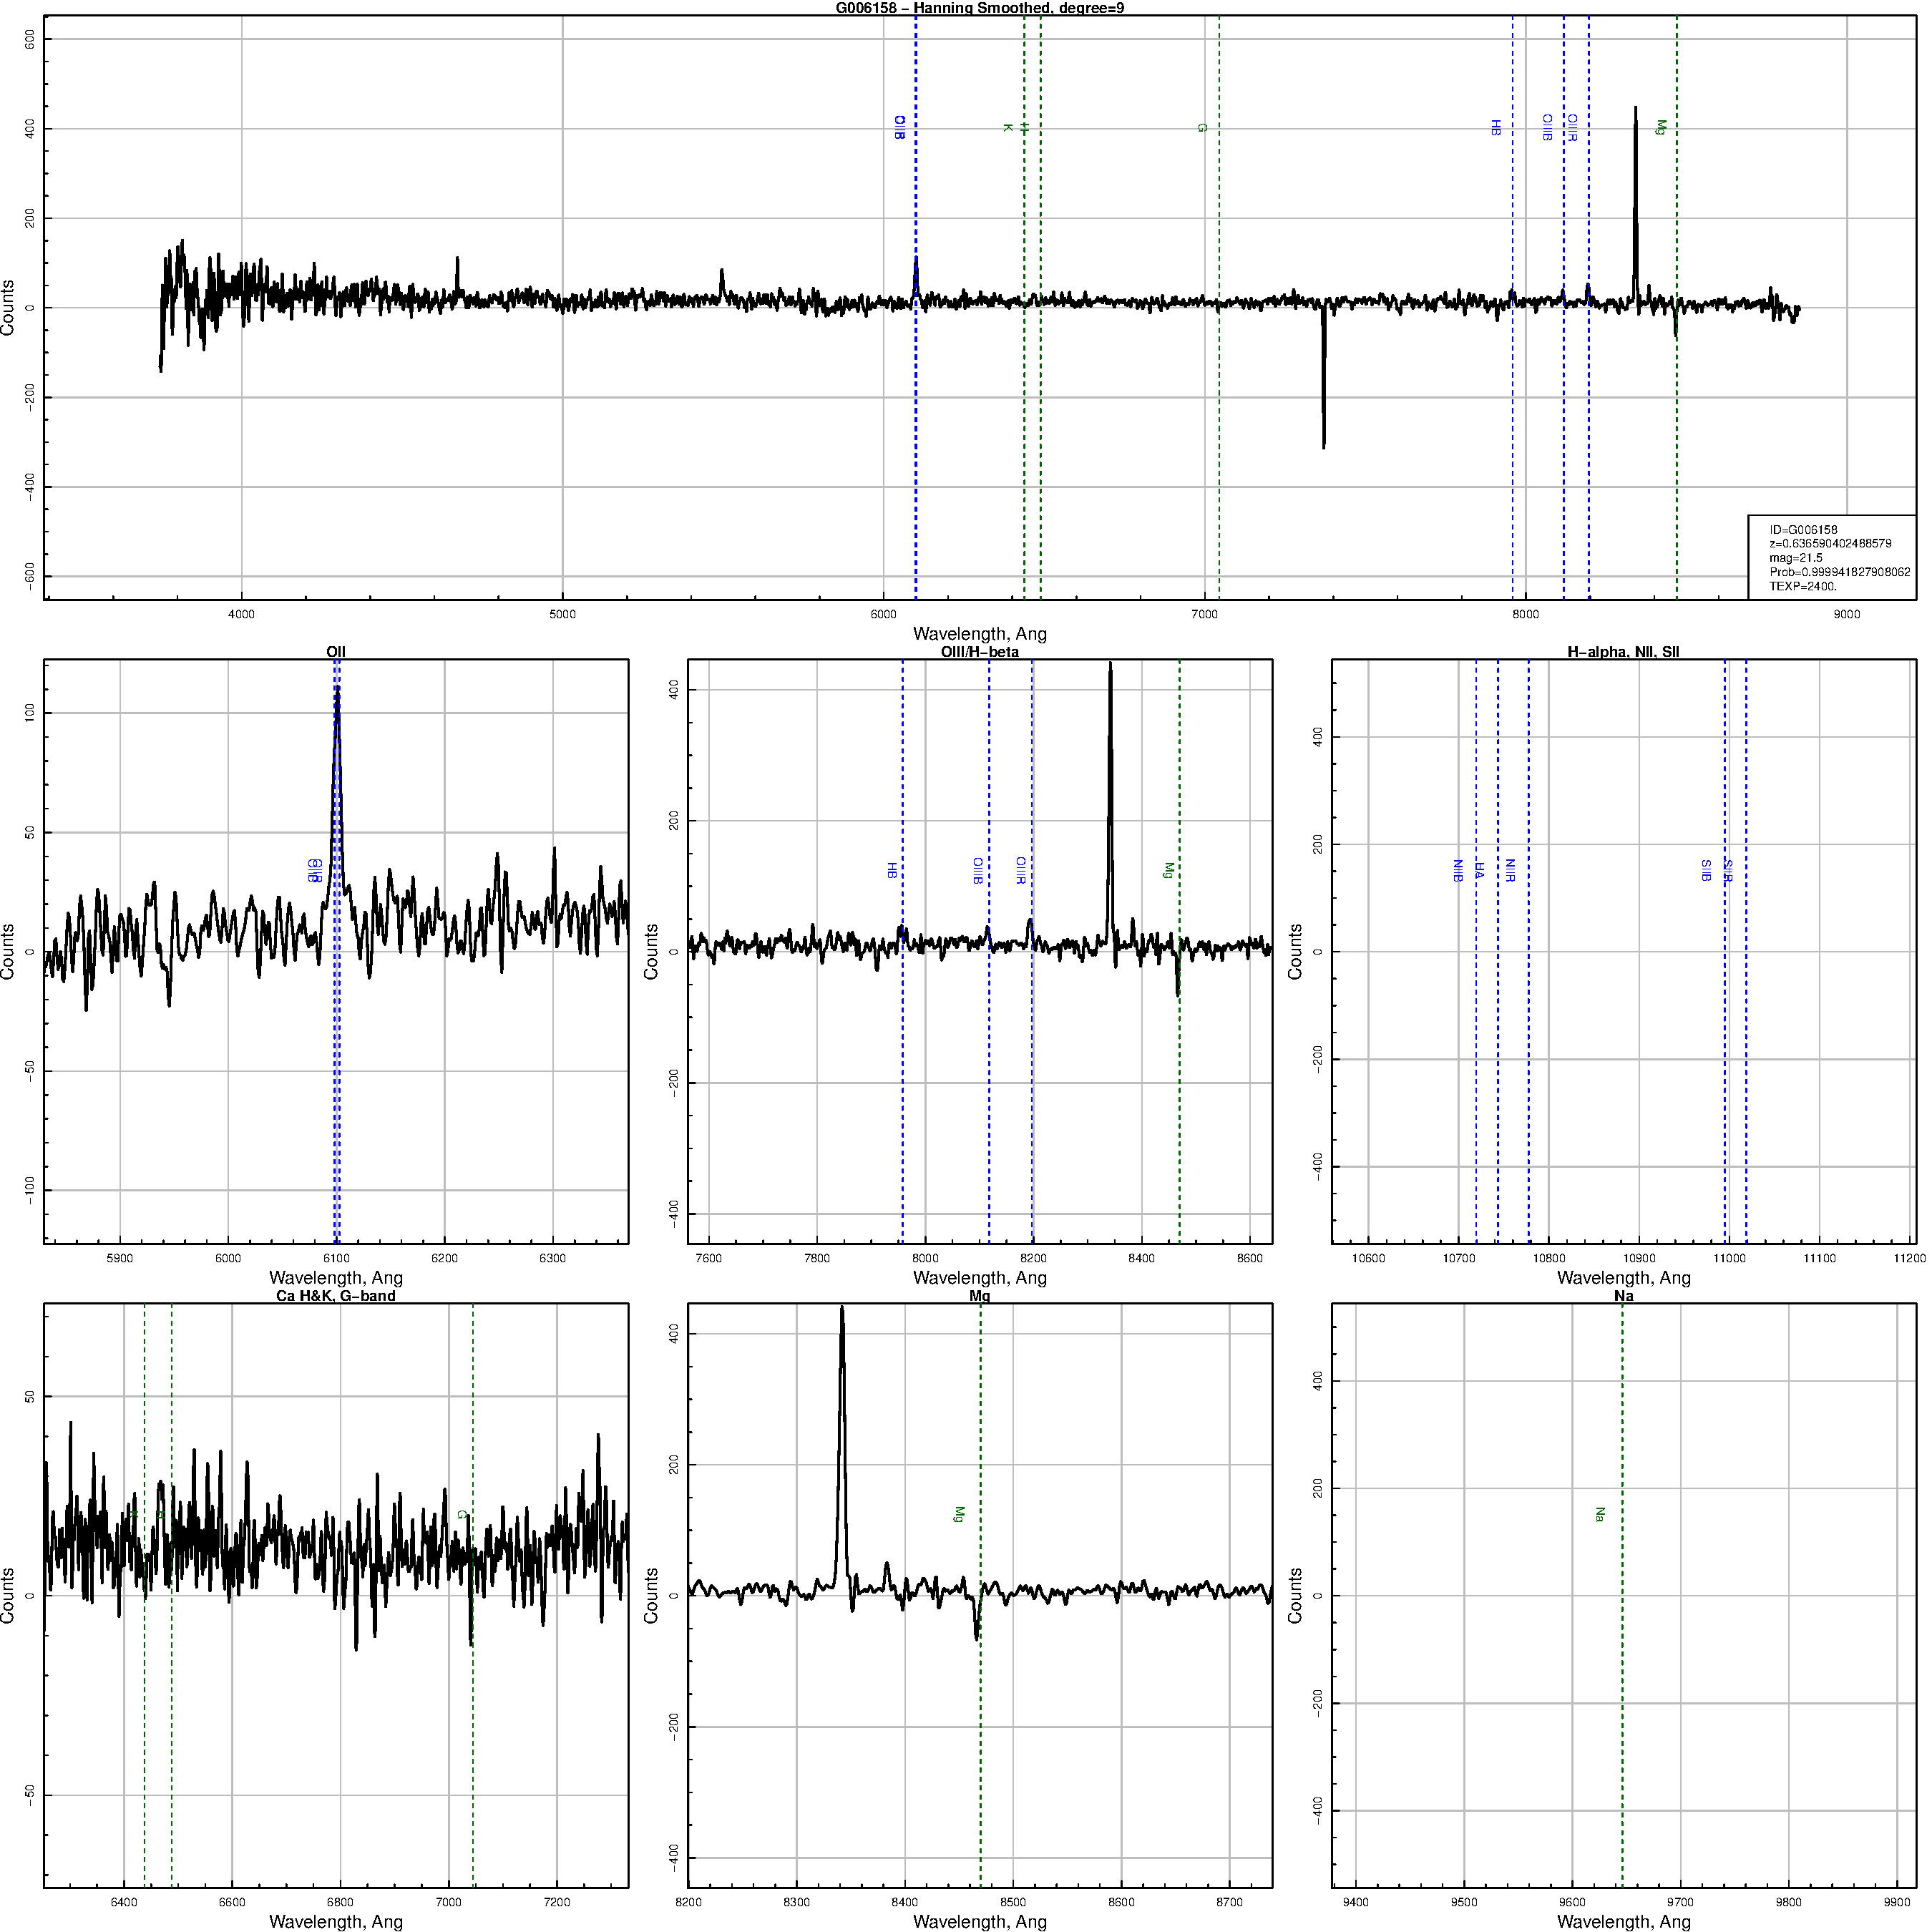
\includegraphics[scale=0.4]{G006158.pdf}
\caption{Example output of TAZ after running AutoZ. Top row shows the full spectrum, middle row shows the location of key emission features at the source's measured redshift, and the bottom row shows the same but for absorption features. Line positions at the fitted redshift are shown as dashed vertical lines (emission in blue and absorption in green). Details of the fitted redshift are given in the legend of the top panel. All spectra are Hanning smoothed.}
\label{fig:specEx}
\end{center}
\end{figure}


\section{Brave TAZ Data Reduction}

If you are feeling particularly brave, you can try an run the reduction automatically using TAZ. \textbf{\textcolor{PineGreen}{PLEASE DO THIS ON YOUR LAPTOP AS NOT TO OVERWRITE FILES IN THE MAIN DATABASE}}. If you have TAZ set up on your laptop (see the document TAZ\_Manual.pdf). Fistly, if you haven't done so you will need the directory structure set up on your laptop. You can do this by opening an R session and running:\\

\texttt{$>$ setUpDir (runs = c(`run\#\_YYYY\_MM'), dateStart = c(`YYYY\_MM\_DD'), dateEnd = c(`YYYY\_MM\_DD'), verbose = 1)} \\

With the run, and date replaced with the current date. In this example, we will use the first DEVILS observing date, run as:\\

\texttt{$>$ setUpDir (runs = c(`run1\_2017\_12'), dateStart = c(`2017\_12\_18'), dateEnd = c(`2017\_12\_18'), verbose = 1)} \\

 This will set up the correct TAZ directory structure, just for the current night. Now, you will need to copy the raw bias, dark and target files (arc, flat, sources) to the correct directories:\\

biases $->$ \textbf{/data/biases/run1\_2017\_12/}\\
darks $->$ \textbf{/data/darks/run1\_2017\_12/}\\
target files $->$ \textbf{/data/raw/run1\_2017\_12/2017\_12\_18/}\\

You can then simply run TAZ as:\\

\texttt{$>$ TAZ(user=*yourname*, workingDir='.',verbose=2, doReduce=T, doExtract=T,  \\ doStack=T, doAutoZ=T, cores=*number of cores to run*, doUpdateMaster=F, \\ doTiler=F, zeroPoint=F)} \\

This will then perform the reduction and extraction and populate the directory structure. You can then look at the reduced and extracted 1D spectra in \textbf{data/reduced/run1\_2017\_12/2017\_12\_18/ \\ stackedSpec/AutoZplots/ }. As you will only be running a single nights data, all spectra will only have one spectrum in their stack. 


\section{Observing Tasks and Checklist}
\label{sec:summary}

In general (assuming nothing goes wrong!) the observer will perform the following tasks:\\

\begin{enumerate}

\item Ensure that the support astronomer takes $\sim30$ bias frames and $\sim30$$\times$20 minute long exposure darks at the start of the run.

\item Copy bias and dark frames to the correct directories on the AAT database and ADC database. 

\item Examine bias and dark frames for QC. This can be done by running \texttt{checkCal()}. Copy and bad frames to the \textbf{junk/} folders.

\item Take .sds and .fld files from the night's \textbf{$\sim$/data/observing/run\#\_YYYY\_MM/YYYY\_MM\_DD/ \\
DOCats/Tiling/TileFiles/} directory and copy them to the \textbf{configs/devils/run\#\_YYYY\_MM/ \\
YYYY\_MM\_DD/} and tell the support astronomer which will be configured first on plates 0 and 1.   \textbf{\textcolor{PineGreen}{This must be done by 4pm local time at the AAT}}.

\item Make a night plan for configurations to observe at a given UT using the observability plots and night plan in the \textbf{$\sim$/data/observing/} directories. Add this to the \textbf{ObsPlan} tool with: 2$\times$1,800sec exposures, and 15min changeover time. 

\item Once the plates are configured, check the 2dF has configured correctly, and if not make adjustments to the .sds and .fld files accordingly. Then note this in the night logs and copy them to the directory given above. 

\item Add observing details to the night log regarding weather conditions, seeing, etc.

\item Make decisions on observability based on weather and seeing. 

\item Once the first configuration has been observed, reduce the data manually by making MASTER bias and dark frames and running the \texttt{run2dfDR\_AAT} script.   

\item Extract 1D spectra using \texttt{AATExtract()} and inspect.

\item Identify any data errors, move poor data to the correct \textbf{junk/} folder and note in the night log.

\item Add reduction details to night logs.

\item Ensure that all raw data (biases, darks, arcs, flats and targets) are copied to the correct folders in the AAT database and ADC database.

\end{enumerate}

\section{DEVILS Data Flow}
\label{sec:dataflow}

Below the DEVILS data flow, as displayed in Figure \ref{fig:dataflow}, is described in details. In this section all of the stages of the figure will be described to allow the user to follow the data-flow through the diagram. Firstly, lets start at a point where the observations for a night have just been completed, at the bottom of the purple box in the Figure...... \\

$\bullet$ The observer takes the raw data from the \textbf{\$AATDATA/YYMMDD/} directories at the telescope and copies them to the correct files in the AAT database (blue box). This process follows the red arrows in the Figure. \\

$\bullet$ Once all of the data is in the database for a given configuration, the observer can perform the nightly reduction and QC. Ignore the right hand side of the figure for now, and more to the bottom yellow box.

$\bullet$ The observer reduction and QC checks are described on the left hand side of the yellow box (led by the white arrow). This is a self contained loop, which describes the observer moving bad data to the \textbf{junk/} folders and updating logs.\\

\hspace{10mm} - The observer checks the raw calibration data quality using the \texttt{checkObs()} function and moves any bad data to the relevant \textbf{junk} folder.\\

\hspace{10mm} - The observer then performs manual data reduction using \texttt{run2dfDR} and populates the \textbf{data/reduced \_AAT} sub-folder. \\

\hspace{10mm} - The observer then performs QC checks on the reduced 2D data frames\\

\hspace{10mm} - The observer then extracts 1D spectra using  \texttt{AATExtract()} and performs QC checks.\\

\hspace{10mm} - The observer updates all night logs with any relevant information.\\

$\bullet$ At the end of each night, once poor data has been moved to the relevant \textbf{junk/} folders, the raw data is synced to the ADC database (purple lines from blue to orange box) and then synched to Perth (purple lines from orange to green box). \\

$\bullet$ During the day, TAZ is run over the new raw data in the Perth Archive. \\

\hspace{10mm} - TAZ makes master darks and biases, if required.\\

\hspace{10mm} - TAZ reduces target data and populates the \textbf{data/reduced} folders. \\

\hspace{10mm} - TAZ extracts 1D spectra, and populates the \textbf{data/reduced/.../..../*config\_\#*/} and \textbf{data/ reduced/allSpec} directories. \\

\hspace{10mm} - TAZ stacks all observations of the same source and populates the \textbf{data/reduced/stackedSpec} folder. \\

\hspace{10mm} - TAZ runs AutoZ over all stacked spectra, updates the meta information in the \textbf{data/reduced/ stackedSpec} folder and populates the \textbf{data/reduced/stackedSpec/AutoZplots/} folder. \\

\hspace{10mm} - TAZ updates the DMCat with new redshifts (generating a new, date-stamped catalogue) and writes to  \textbf{data/catalogues/DMCats/} \\

\hspace{10mm} - TAZ reads the new DMCat and generates a new set of DOCats in \textbf{data/observing/.../.../DOCats/}  \\

\hspace{10mm} - TAZ generates new fibre configuration files using the DOCats but running \textsc{configure} and writes these files to the \textbf{data/observing/.../.../DOCats/Tiling/TileFiles/} directory. \\


$\bullet$ The reduced and observing directories are synced back to the AAT via ADC (orange arrows from green, orange then blue boxes).\\

$\bullet$ The observer collects the configuration files from the \textbf{data/observing/.../.../DOCats/Tiling/TileFiles/} directory, checks files and makes night plan as shown by the purple arrows leading through the right hand side of the yellow box.\\ 

$\bullet$ The observer passes the configuration files to the support astronomer via the \textbf{configs/} directory. \\ 

$\bullet$ The support astronomer configures 2dF (top of purple box). \\

$\bullet$ If there are any issues with configuration, the observer manually amends the configuration files (top yellow box within purple box).\\

$\bullet$ AAT observations are undertaken. During this time the observer makes decisions on fields to observer, when to stop observing because of poor weather, etc.  \\

$\bullet$ Raw data from the observations is copied to the \textbf{\$AATDATA/YYMMDD/} directories. And repeat. 

\begin{figure}
\begin{center}
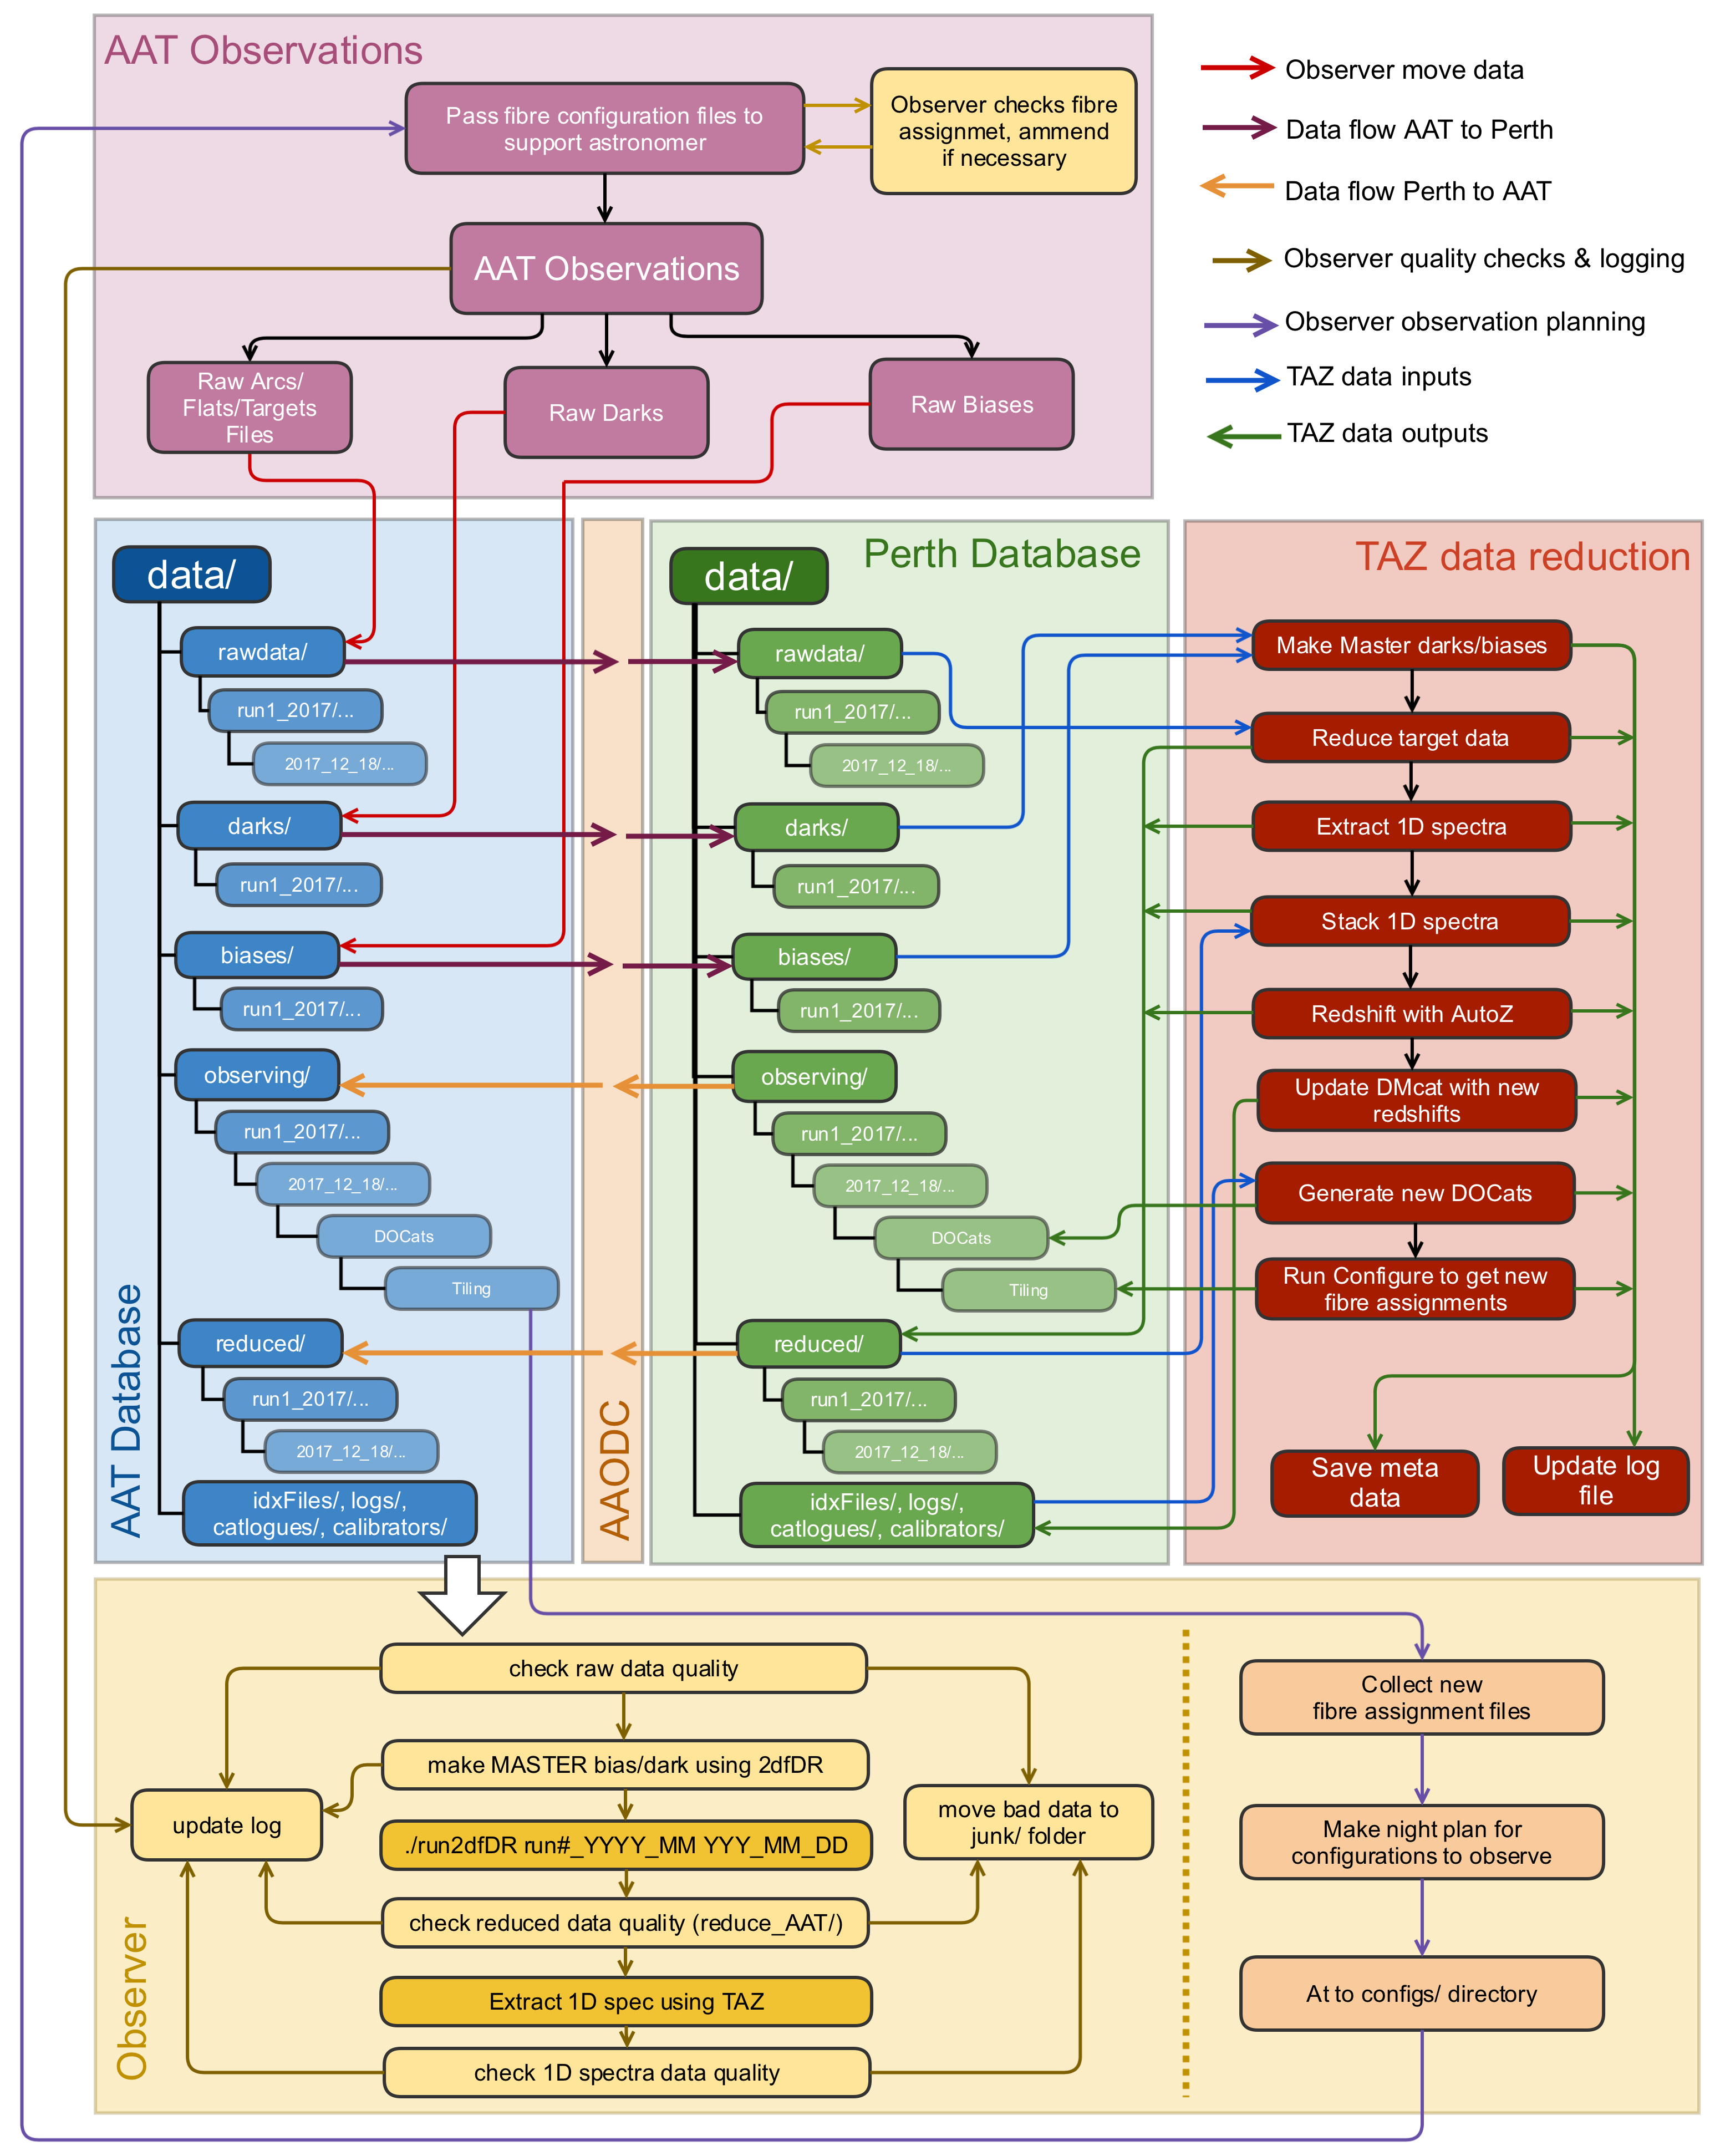
\includegraphics[scale=0.17]{devils_taz_dataflow.png}
\caption{DEVILS survey data flow}
\label{fig:dataflow}
\end{center}
\end{figure}


\end{document}

